\section{Introduction}
\label{sec:Intro}

The advent of cloud computing and the Internet of Things (IoT) has led to a massive rise in the demand for online data storage and data sharing services. Two very important paradigms that any data sharing service provider must ensure are privacy and flexibility. Since online data almost always resides in shared environments (for instance, multiple virtual machines running on the same physical device), ensuring privacy is a non trivial task. Current technology for secure data sharing comes in two major flavors - trusting a third party auditor \cite{cryptoeprint:2009:579} or using the user's own key to encrypt her data \cite{chow2012dynamic}. Figure \ref{fig:intro} describes a realistic online data sharing set-up. Suppose a data owner stores multiple classes of encrypted data online with the intention of providing users decryption keys to one or more such ciphertext classes, based on their respective credentials. She might also wish to dynamically update the delegated access rights based on 
changes to the data/credibility issues. The challenge therefore is to provide her with a secure and efficient online data sharing scheme that allows updates to user access rights on the fly. 


A n\"{a}ive (and extremely inefficient) solution is to have a different decryption key for each ciphertext class, and share them accordingly with users via secured channels. A more efficient proposition is the key-aggregate encryption (KAC) scheme proposed in \cite{chu2014key} that combines the power of individual decryption keys, for ciphertext classes in a given subset, into a single key for that subset. This key is specific to the designated subset, meaning that it cannot be used to decrypt any ciphertext class outside that subset. KAC derives its roots from the seminal work by Boneh \textit{et.al.} \cite{boneh2005collusion} that allows broadcasting of data (encrypted by the same public key) among multiple users, each of whom possess their own private keys for decryption. Both these schemes make use of bilinear mappings on multiplicative cyclic groups. 

 
 \begin{figure}[!t]
\centering
\captionsetup{font=scriptsize}
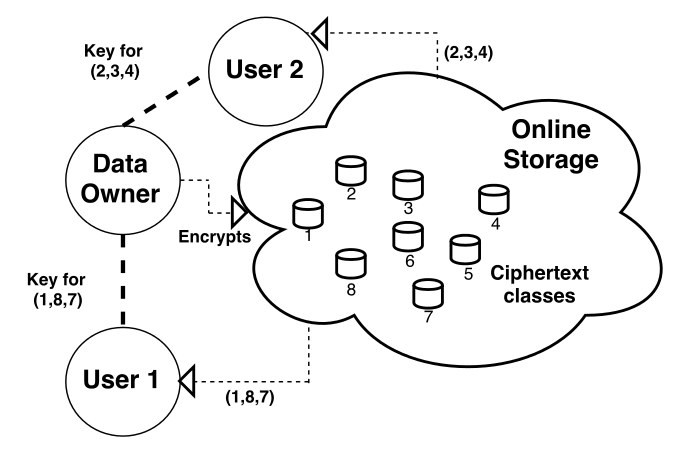
\includegraphics[scale=0.25]{Figs/KeyAgg.png}
\caption{Example of Online Data Sharing}
\label{fig:intro}
\end{figure}


\noindent{\textbf{Contributions:}} In this paper, we propose a basic key-aggregate scheme on additive elliptic subgroups that delegate decryption rights to multiple ciphertext classes using a single constant sized key. The scheme is dynamic in nature, that is, it allows the data owner to revoke access rights of users without having to change the entire set-up, unlike in the existing KAC scheme.  We then generalize this scheme into a two-level construction that allows flexible public key extension and maintains constant ciphertext size, while avoiding many of the pitfalls of earlier hierarchical schemes. We provide a formal proof of semantic security for the generalized scheme. We further extend the generalized scheme to allow using popular and efficiently implementable elliptic curve pairing schemes. We compare the time and space requirements of the proposed generalized scheme under various operating configurations. We also compare the performance of our proposed scheme, in terms of key size and resource 
utilization, with that of other existing schemes in literature.

\noindent{\textbf{Organization:}} The rest of the paper is organized as follows. Section \ref{sec:relwork} provides a brief overview of state of the art data sharing schemes. Section \ref{sec:prelims} introduces the notion of key aggregate cryptosystem, and provides a description of the complexity assumptions used to prove the semantic security of our proposed schemes. Our basic dynamic key-aggregate scheme is presented in Section \ref{sec:proposal}. We follow up with a more generalized two-tiered construction of the scheme for efficient public key extension in Section \ref{sec:general}, and prove its semantic security. A further extension for the generalized scheme that allows using efficiently implementable pairings is introduced and proved semantically secure in Section \ref{sec:extended}. Experimental results using Tate pairings based implementations of the extended scheme are presented in Section \ref{sec:results}. Finally Section \ref{sec:conclusions} concludes the paper.  


